\section{Proposed Solution}
The problem of Boolean Function Synthesis can be posed as a learning problem. 
In an abstract sense, Observations O corresponds to boolean relational formula 
that serves as the specification for synthesizing skolem function.

let, F = Relational Specification (Observations)

\tab $\psi$ = Skolem Function Vector (Target)

And the aim is to learn a hypothesis function $'h'$ 

s.t.  $h(F;\hat{\theta}) = \hat{\psi}(X)$, where $\theta$ are learneable parameters of the model and
X denotes the set of input variables from the observations.

For a given dataset $\mathcal{D} = {(f_i, \psi_i)|1 \leq i \leq N}$, we want to minimize the 
expected loss between $\hat{\psi}(X) and \psi$

$$\text{Expected Loss: } E(l(\hat{\psi}(X), \psi)) \approx \frac{1}{N} \sum_{i=1}^{N} l(\hat{f_i}, \psi_i) $$

$$\hat{\theta} = \underset{\theta}{argmin} \frac{1}{N} \sum_{i=1}^{N} l(\hat{\psi_i}, \psi_i)$$

We model h using GCLN \ref{gcln}. 
The parameters in this network are the Gates ($\theta = (G_1, G_2)$) which acts like a switch 
for the input variables ($G_{1}$) or clauses ($G_{2}$).

As $\psi$ is not known to us, training a neural net over (F, $\psi$) is not possible. Therefore,
we perform sampling over
the boolean variables in formula F and mark the set of input variables (X) as the features and 
the set of output variables 
(Y) as the ground truth labels. Sampling strategies are discussed in detail in section \ref{sample}.

Sampling is done such that it captures the relation between X and Y. We exploit this fact and learn 
a function mapping $\psi$: X \rightarrow Y, wihch is our end goal.

We have implemented 4 different algorithms for solving this problem. We discuss these in the next section
\ref{algo} .

% If m is the number of input variables then 2*m is the size of each clause.



\section{Problem Formulations}\label{algo}
As of now we have come up with 4 different formulations for training the network. 
In this section we discuss those formulations. 
We also discuss their performance over a small set of toy examples.

\subsection{Regression}
This uses Random Sampling Strategy \Romannum{1}. Training data contains only positive samples. 
Output variables (Y) of the specification are the target variables while the input variables (X) are the features.
As the target values are real, most intuitive thing is to do regression.
The GCLN model regresses over the output variable. Loss function used here is mean square error loss.

Figure \ref{fig:regr} pictorially describes the algorithm.


\noindent\textbf{Intuitive Explanation for its Working: } With the given set up, model learns to predict Y's given X's.
That is it learn a function mapping from X to Y and this is the definition of the desired function to be synthesize. 
Now because we had sampled only samples which made the specification True, the function learnt for Y will output only 
those truth values of Y which would make the specification True.

\begin{figure}
	\centering
    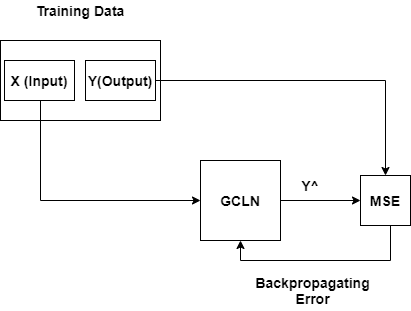
\includegraphics[scale=0.4]{regression.png}
    \caption{Regression Formulation}
    \label{fig:regr}
\end{figure}

\subsection{Classification Problem - 1}
Using Random Sampling Strategy \Romannum{1} we sample the training data.
In this case, the sampled real valued output variables (Y) are converted to binary ($Y_{bin}$) based on given threshold. 
Now we can consider $Y_{bin}$ as the class labels and learn a classifer over them. 
Loss function used in this case is Binary Cross Entropy Loss.

Figure \ref{fig:class1} describes it pictorially.

\noindent\textbf{Intuitive Explanation for its Working: } If the model learns a best fit
separating hyperplane, it will predict class labels $Y_{bin}$ for X. Which essentially means that the classifier is 
a mapping from X to $Y_{bin}$. As the data consists of only positive examples, the classifier would 
represent the required function.

\begin{figure}
	\centering
    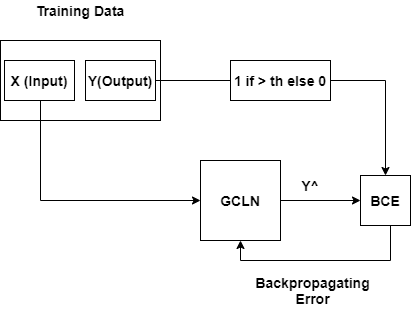
\includegraphics[scale=0.4]{class1.png}
    \caption{Classification - 1}
    \label{fig:class1}
\end{figure}

\subsection{Classification Problem - 2}\label{class2}
We use Random Sampling Strategy \Romannum{2}. Training data is $(X, F_{out})$ pairs, where, $F_{out}$ is the
output of F for the sampled input variables (X) and output variables (Y). i.e. X is features and $F_{out}$ 
are the class labels. Once $F_{out}$ is computed, Y is discarded.
While training we take the output of GCLN model $\hat{Y}$ and the input variables $X$ from trainig data
 and compute the value of $\hat{F_{out}}$ over them. In this set up, $\hat{Y}$ is the latent variable that 
 the model learns to predict. Loss function used is Binary Cross Entropy Loss over $\hat{F_{out}}$ and $F_{out}$
Figure \ref{fig:class2} descibes this pictorially.

\begin{figure}
	\centering
    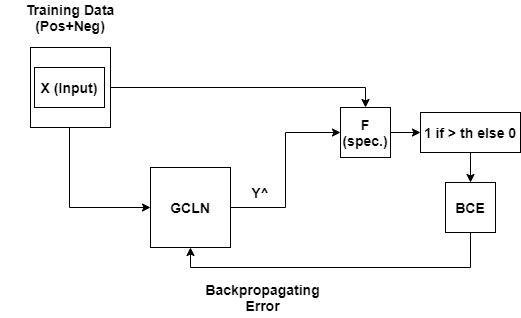
\includegraphics[scale=0.4]{class2.png}
    \caption{Classification - 2}
    \label{fig:class2}
\end{figure}

\noindent\textbf{Intuitive Explanation for its Working: } Here the model learns to predict correct $F_{out}$.
For that it first learns the latent variable $Y$ given only $X$ as its input. So, the model would learn a classifier
that tells which $Y$ to output such that it correctly classifies the $F_{out}$. It means that model will act as a 
mapping from X to Y such that it matches $F_{out}$ and $\hat{F_{out}}$. As the output of classifier mimics Y
for given X, it should represent the required skolem function.

\subsection{Classification Problem - 3}
This is same as \ref{class2} except the sampling strategy used here is correlated sampling
explained in \ref{sample3}.

\section{Extraction Algorithm}
\noindent\textbf{Number of input variables = n, Number of output variables = m, Maximum clauses = K
Gates in Disjunction Layer - G1 ($2n \times mK$)
Gates in Conjunction Layer - G2 ($mK \times m$)}
\\
1. Input Vector I = [input variables, ~(input variables)]\\
if there are n input variables then Input Vector I, would be of size $2n \times 1$
\\
2. Apply gates G1 and construct mK clauses each of size 2n where m is the number of output variables.
\\
3. Apply gates G2 and select suitable clauses for each output variables. First K clauses corresponds to the first output variable, 
second K clauses corresponds to the second output variable, and so on.
\\
4. Finally, we have boolean formula for each output variable in terms of input variables.

\section{Results}
The output variable in the specification is replaced with the extracted formula from the network and checked for validity using z3Py Solver.
Figure \ref{fig:results} shows the preliminary results over 5 toy problems. The results are not very impressive at the moment but the hope 
is with intelligent sampling and better training procedure, this can be improved.

\begin{figure*}
	\centering
    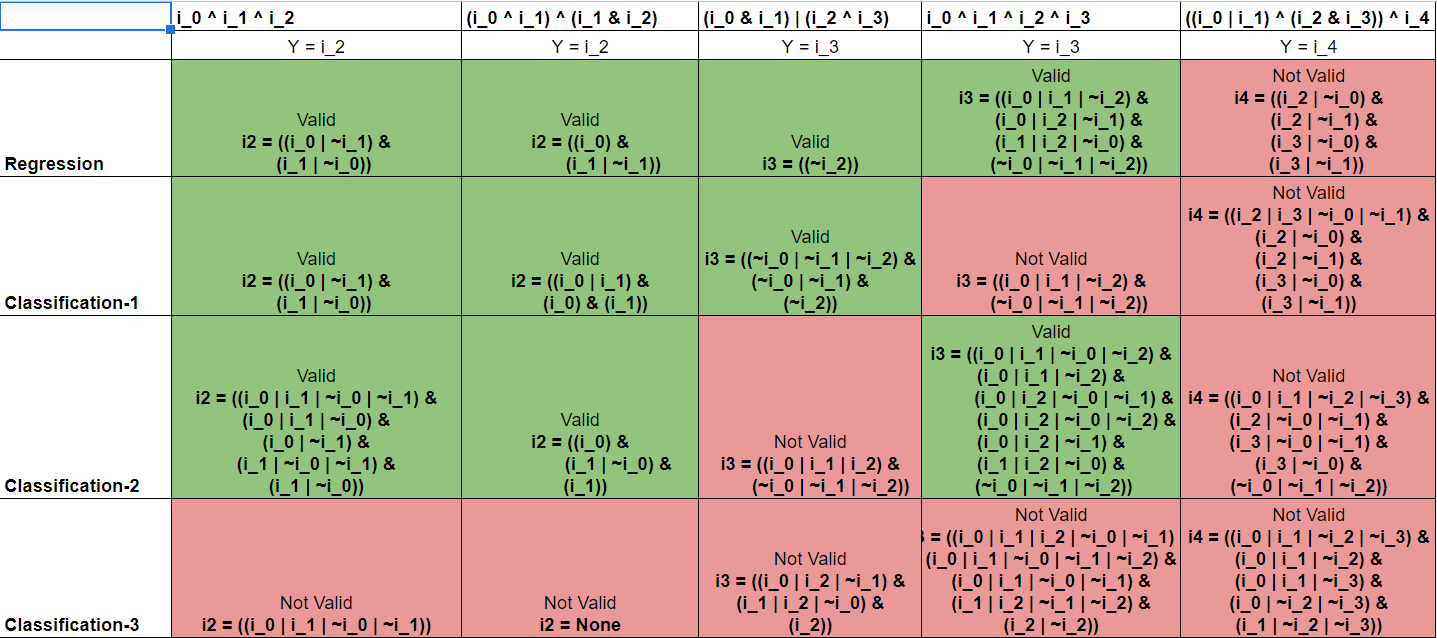
\includegraphics[scale=0.5]{results.png}
    \caption{Results on 5 toy Problems}
    \label{fig:results}
\end{figure*}